\chapter{Visor web dinámico de objetos 3D}\label{cap.visor3d}
En este capítulo se va a tratar la creación de un nuevo visor de elementos 3D (modelos, puntos y rectas) con tecnologías web. Este visor, al que se ha nombrado como 3DVizWeb, nos abrirá la posibilidad de obtener datos por una cámara o sensor y mostrar una representación 3D de los mismos.
\section{Diseño}
Este visor está elaborado usando JavaScript y HTML como lenguajes de programación, y se usará el middleware ICE para la interconexión con los clientes que nos enviaran los datos a mostrar. A continuación se muestra una imagen con el diseño del visor 3D:

\begin{figure}[H]
  \begin{center}
    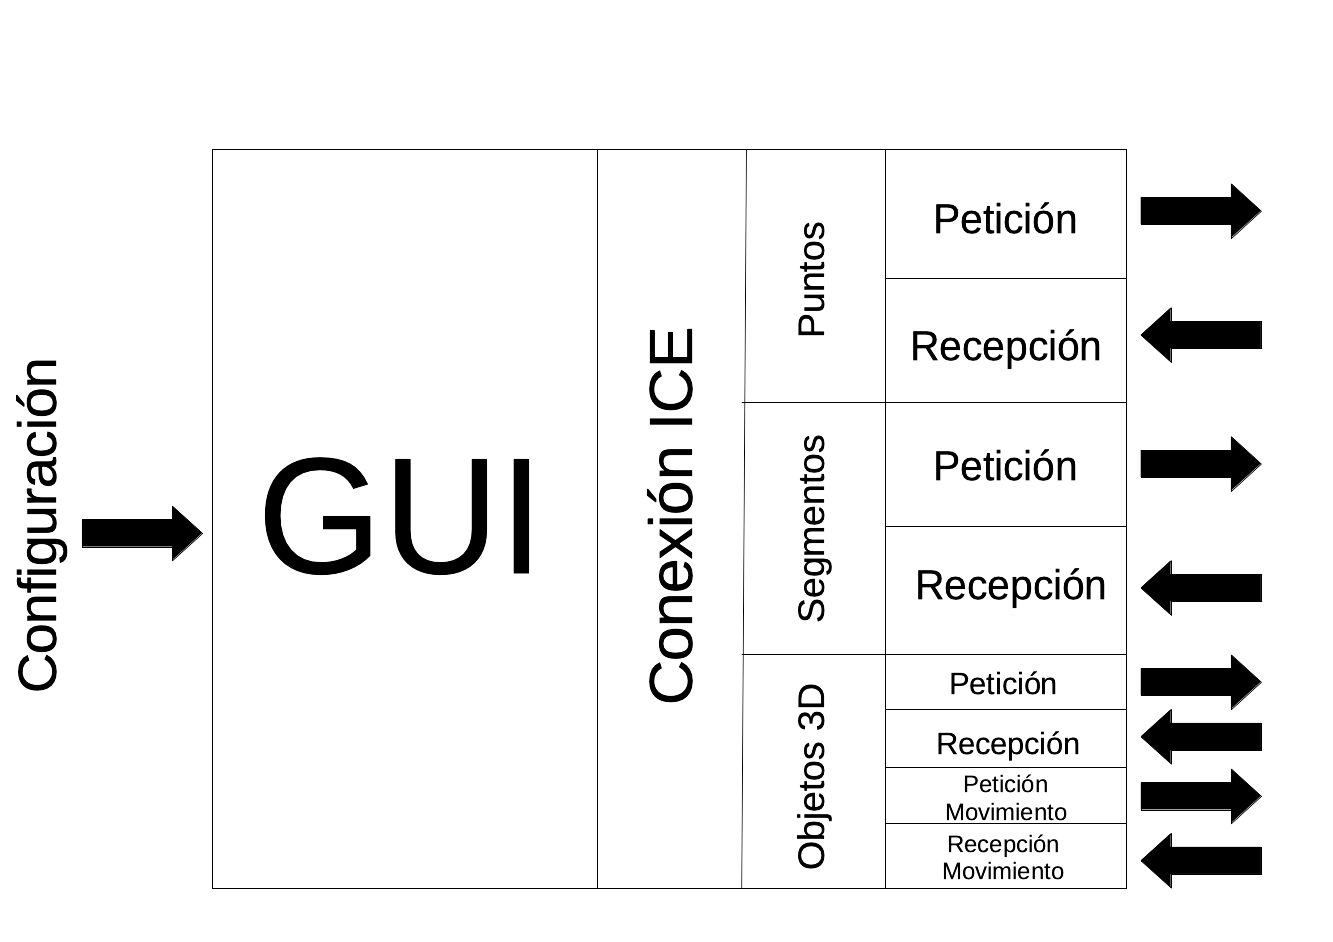
\includegraphics[width=0.8\textwidth]{figures/diseno3dviz.png}
		\caption{Diseño del visor 3D}
		\label{fig.diseno3dviz}
		\end{center}
\end{figure}
La herramienta esta dividida en dos partes: la interfaz gráfica y las conexiones ICE.

La parte correspondiente a la interfaz gráfica será la que da origen a nuestro visor y cómo se definen cada uno de los tipos de objetos que es capaz de mostrar, para que la interfaz sea capaz de mostrar todos los objetos recibidos desde el servidor.

Las conexiones ICE con el servidor incluyen a su vez varias partes claramente sementadas. Estas partes corresponden a la petición y recepción de cada tipo de elemento al servidor, haciendo especial hincapié a los objetos 3D que contarán con las peticiones y recepciones para mostrar nuevos objetos y otras peticiones y recepciones de movimiento de los objetos 3D que ya se están mostrando.

\section{Configuración}
En este apartado se va a explicar el método utilizado para configurar el visor 3D. Dado que el visor en su interfaz gráfica únicamente muestra la escena donde se mostrará los objetos como se explicará en la siguiente sección, es necesario utilizar una alternativa para configurar los datos de conexión (ip y puerto de escucha) y otros parámetros configurables (posición inicial de la cámara, tamaño de los puntos, tamaño de los segmentos y periodo de tiempo entre peticiones de cada tipo de objeto) antes de arrancar el visor.
Se ha decidido usar un archivo externo con formato ``YAML'' que será leído y cargada la información por el visor al arrancar. ``YAML'' es un formato de serialización de datos muy sencillo de usar y de leer por una aplicación. Usando una única línea de código, somos capaces de cargar y guardar en una variable la información que contiene un archivo de este tipo. Para cargarlo en el visor, vamos a usar el siguiente código:
\begin{lstlisting}[frame=single]
const yaml = require('js-yaml');
const fs = require('fs');
config = yaml.safeLoad(fs.readFileSync('config.yml', 'utf8'))
\end{lstlisting}
Con este código, habríamos cargado el contenido del archivo ``config.yml'' (``.yml'' es la extensión de ``YAML'') en la variable ``config''.

Los parámetros que podrán ser configurados en el visor serán los siguientes:
\begin{itemize}
\item Dirección IP. Por defecto será ``localhost''
\item Puerto. Por defecto será ``11000''
\item Tiempo de refresco para la petición de puntos en milisegundos. Por defecto serán 1000 ms
\item Tiempo de refresco para la petición de segmentos en milisegundos. Por defecto serán 1000 ms
\item Tiempo de refresco para la petición de objetos 3D en milisegundos. Por defecto será 1 ms
\item Tiempo de refresco para la petición del movimiento en milisegundos. Por defecto serán 1000 ms
\item Grosor de los segmentos en pixeles. Por defecto serán 2 pixeles.
\item Tamaño de los puntos en pixeles. Por defecto serán 8 pixeles.
\item Posición inicial de la cámara. Estará formada por ``x'', otra ``y'' y ``z'', siendo por defecto ``50'', ``20'' y ``100'' respectivamente.
\end{itemize}

\section{Interfaz gráfica}
La interfaz gráfica del visor está diseñada usando WebGL, y más concretamente usando la biblioteca Three.js descrita en capítulos anteriores.La interfaz será íntegramente el visor (no tendrá ningún elemento adicional), el cual mostrará inicialmente una rejilla que hará de plano horizontal, cuyo centro será la posición (0, 0, 0) del eje de coordenadas. Además es necesario añadir iluminación y una cámara para poder visualizar la escena.

\subsection{Escena base}
El visor está contenido dentro de un elemento HTML <canvas>. En este elemento se crea una nueva escena usando la función de Three.js THREE.Scene() y se renderiza usando THREE.WebGLRenderer(). Posteriormente se crea una cámara perspectiva utilizando THREE.PerspectiveCamera() ubicándola en una posición predeterminada (la indica en el archivo de configuración anteriormente indicado)y podrá ser controlada mediante teclado o ratón. Finalmente, para visualizar correctamente la escena se añaden varias luces puntuales a lo largo de la misma, así como una iluminación de ambiente utilizando THREE.PointLight() y THREE.AmbientLight() pasándole como parámetros el color de la luz y la intensidad de la misma.


Una vez tenemos una escena completamente visible, se procede a crear y añadir la rejilla. La función existente en la biblioteca Three.js, new THREE.GridHelper(), nos permite definirla muy fácilmente introduciendo por parámetro a la función la separación, cantidad y color de las líneas de división que generan la rejilla. Para añadirla a la escena, bastará con usar .add(rejilla). Estos elementos formaran la escena base del visor.

\begin{figure}[H]
  \begin{center}
    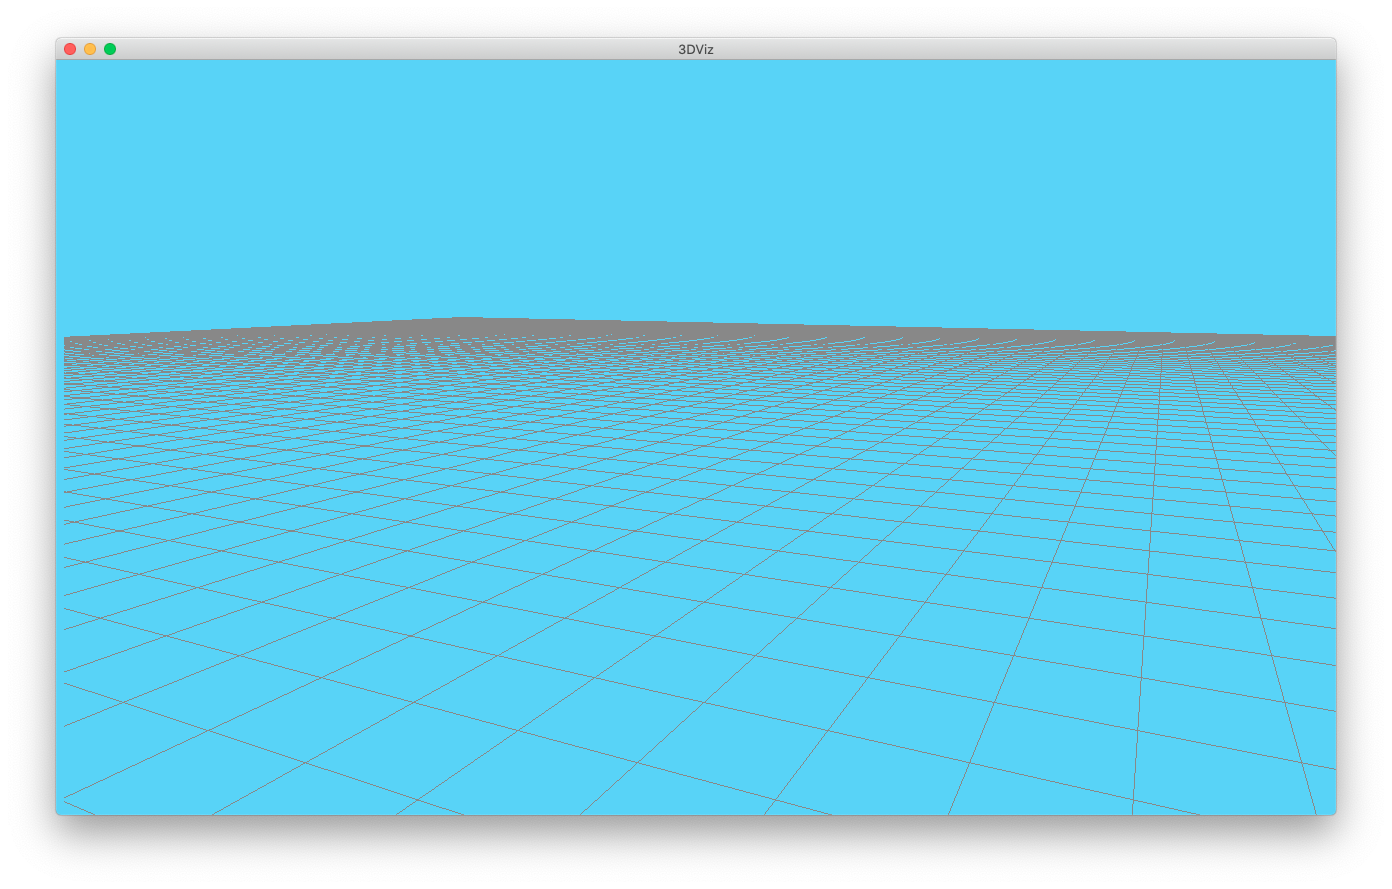
\includegraphics[width=0.8\textwidth]{figures/interfazinicial.png}
		\caption{Interfaz gráfica base del visor}
		\label{fig.interfazinicial}
		\end{center}
\end{figure}

\subsection{Visualizar puntos}
Un punto es el elemento geométrico más simple que es posible representar. Sin embargo, pese a ello, proporciona a nuestro visor la capacidad de realizar representaciones más complejas mediante el uso de una gran cantidad de puntos. Para representar puntos, únicamente es necesarios una posición en el eje de coordenadas, el tamaño del punto y el material o color que queramos darle. 
La biblioteca Three.js nos proporciona una serie de elementos para facilitar la creación de puntos. A continuación se muestra el código para crear y mostrar un punto:
\begin{lstlisting}[frame=single]
function addPoint (point){
	var geometry = new THREE.Geometry();
	geometry.vertices.push( new THREE.Vector3(point.x,point.z,point.y));
	var material = new THREE.PointsMaterial( { size: 8, sizeAttenuation: false, 
										alphaTest: 0.5, transparent: true } );
	material.color.setRGB( point.r, point.g, point.b);
	var particles = new THREE.Points( geometry, material );
	particles.name ="points";
	scene.add( particles );
}
\end{lstlisting}
Primero es necesario indicar que estamos creando una figura geométrica para posteriormente definirla. Al tratarse de un punto, solo va a tener un vértice por lo que al definir la geometría indicaremos que serán vertices pero únicamente se proporciona uno de ellos mediante un vector ``x'', ``y'' y  ``z'', el cual serán las coordenadas centrales del punto que queremos representar. Cabe destacar que dado que el sistema de coordenadas de obtención de los datos no se corresponde con el sistema de coordenadas de la escena, hay que realizar una conversión de modo que si recibimos un punto con coordenadas (x,y,z), en la escena corresponderán a (x,z,y). 


Una vez definida la geometría, lo siguiente es definir el tamaño del punto, su aspecto y, posteriormente, su color. El tamaño indicado en el código es de 8 pixels, sin embargo este tamaño es configurable a través de un fichero de configuración indicado en la sección anterior. El color del punto se definirá mediante sus componentes RGB que como se ha indicado anteriormente, vienen indicadas por el servidor que nos transmite el punto. Las componentes vendrán separadas en ``R'', ``G'' y ``B'', y su valor oscilará entre ``0'' y ``1'' (se corresponde con el valor ``255'') para cada una de ellas.


Finalmente creamos el punto a partir de la geometría y el material creado, le atribuimos el nombre ``punto'' para poder borrarlo, si así se desea, y se añade a la escena.
Esta función será invocada cada vez que se reciba uno o más puntos procedentes del servidor. La siguiente imagen muestra varios puntos en el visor:
\begin{figure}[H]
  \begin{center}
    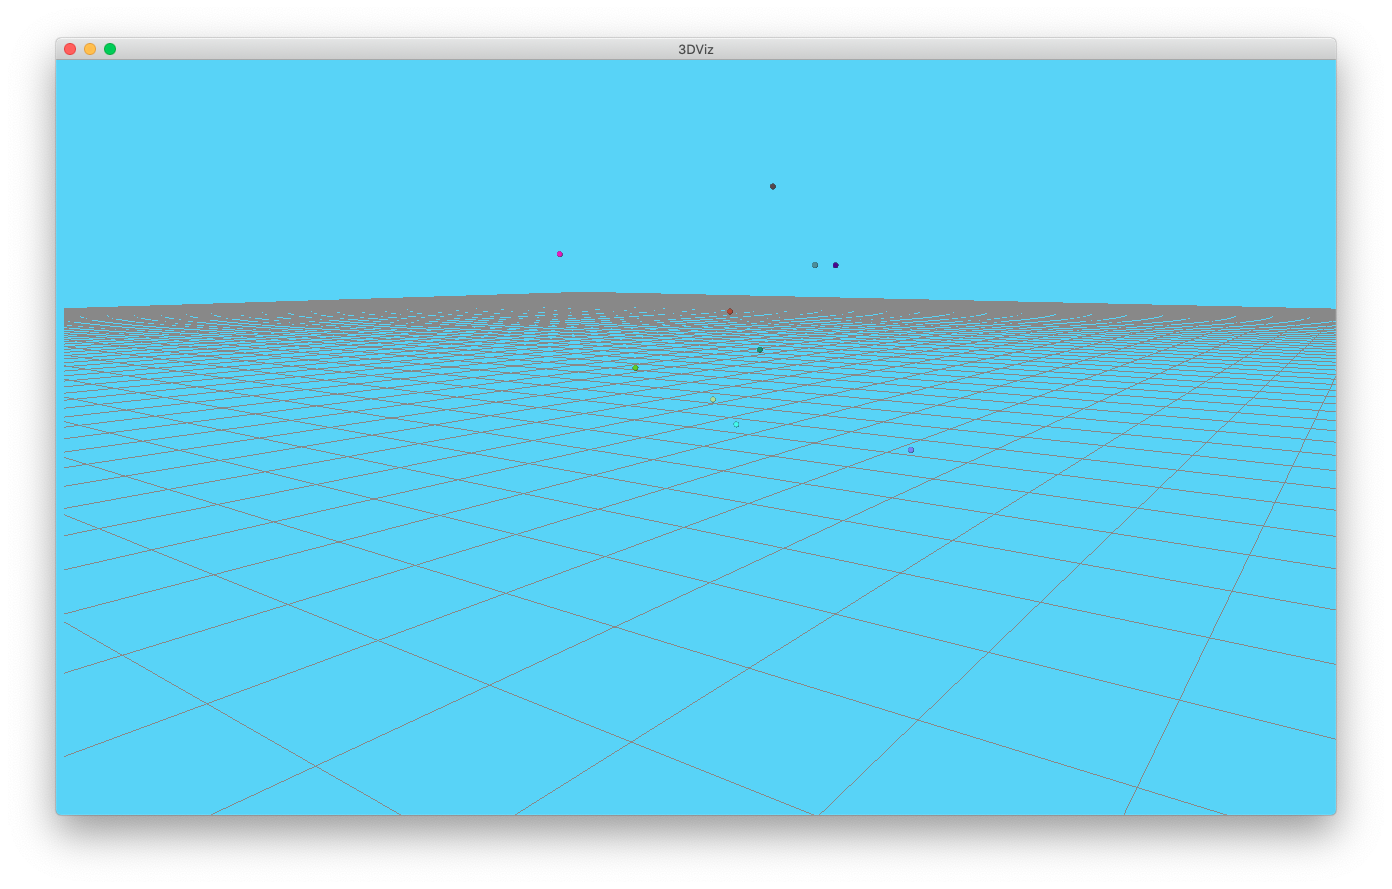
\includegraphics[width=0.8\textwidth]{figures/visualizarpuntos.png}
		\caption{Varios puntos visualizados en el visor}
		\label{fig.visualizarpuntos}
		\end{center}
\end{figure}
\subsection{Visualizar segmentos}
El segmento es otro de los elementos fundamentales de la geometría y se puede definir cómo un fragmento de recta que está comprendido entre dos puntos. Teniendo en cuenta esto, para poder representarlo únicamente es necesario las coordenadas de dos puntos, el grosor del segmento y el color del mismo. A continuación se muestra el código para la creación de una linea:
\begin{lstlisting}[frame=single]
function addLine(segment){
	var geometry = new THREE.Geometry();
	geometry.vertices.push(
		new THREE.Vector3(segment.fromPoint.x, segment.fromPoint.z, 
							segment.fromPoint.y),
		new THREE.Vector3(segment.toPoint.x, segment.toPoint.z, 
							segment.toPoint.y));
	var material = new THREE.LineBasicMaterial();
	material.color.setRGB(segment.r, segment.g, segment.b);
	material.linewidth = 2;
	line = new THREE.Line(geometry,material);
	line.name = "line";
	scene.add(line);
}
\end{lstlisting}
Es fácil de apreciar que la estructura es muy similar que la función para crear un punto. Al igual que para un punto, necesitamos definir la geometría pero, como se ha indicado anteriormente, en este caso vamos a tener dos vértices en lugar de uno (dos puntos), el primer vértice será desde el lugar donde comience la recta, y el segundo vértice, el lugar donde termine, en otras palabras, la recta será la unión entre el primer vértice con el segundo vértice. Las coordenadas de estos dos puntos será proporcionadas por el servidor y, al igual que en el caso del punto, el sistema de coordenadas del servidor no coincide con el sistema del visor, por lo que se debe realizar la misma conversión, es decir la coordenada ``z'' que envíe el servidor, se corresponde a la coordenada ``y'' del visor, y viceversa.

Posteriormente, definimos el material y aspecto del segmento proporcionando el grosor y el color. En el código anterior, el grosor es de 2 pixeles, sin embargo este parámetro será configurable mediante el fichero de configuración explicado anteriormente. El color, por el contrario, vendrá definido por parte del servidor mediante sus componentes RGB, que al igual que para el caso del punto, vendrán sementadas en ``R'', ``G'' y ``B'', valiendo entre ``0''  y ``1'' (corresponde al valor ``255'').

Finalmente se crea el segmento a partir de la geometría y el material creado, dándole el nombre ``line'' para poder borrar únicamente los segmentos, como ya se ha explicado anteriormente. Una vez generado el elemento, se añade a la escena. Esta función será la invocada cada vez que se reciba uno o más segmentos desde el servidor. La siguiente imagen muestra varios segmentos en el visor:
\begin{figure}[H]
  \begin{center}
    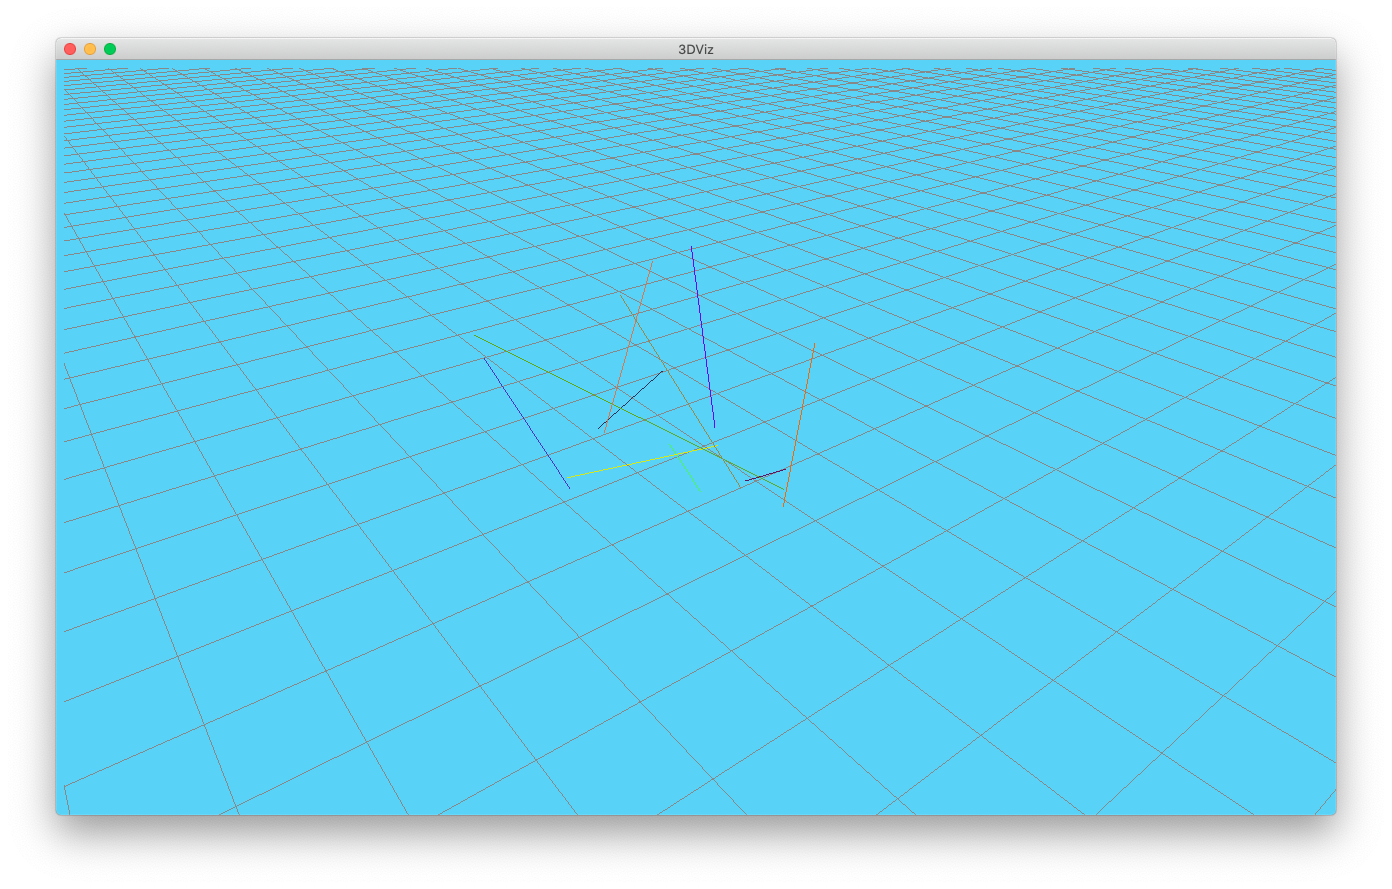
\includegraphics[width=0.8\textwidth]{figures/visualizarlineas.png}
		\caption{Varios segmentos visualizados en el visor}
		\label{fig.visualizarsegmentos}
		\end{center}
\end{figure}

\subsection{Visualizar objetos 3D}
Un objeto 3D es una representación matemática de un objeto tridimensional y que se puede guardar en un archivo de definición de geometría. El visor será capaz de representar dos formatos diferentes de estos archivos, ``obj'' y ``dae'' y moverlos cuando el servidor lo quiera. 

\subsubsection{Creación y visualización de los objetos 3D}
Los objetos 3D podrán ser recibidos o bien a través del archivo completo como texto plano, o bien a través de una url. El visor será capaz de representar el objeto 3D y ubicarlo en la posición indicada. El siguiente código muestra como identificar si el objeto viene como texto plano o url, para posteriormente invocar a la función correspondiente dependiendo el formato del objeto:
\begin{lstlisting}[frame=single]
function addObj(obj,pos){
	var type = obj.obj.split(":");
	if (type[0] == "https" || type[0] == "http") {
		var url = obj.obj
	} else{
		var file = new Blob([obj.obj], {type:'text/plain'});
		var url  = window.URL.createObjectURL(file);
	}
	if (obj.format == "obj"){
		loadObj(url, obj,pos)
	} else if (obj.format == "dae") {
		loadDae(url,obj.pos);
	}
}
\end{lstlisting}
Cuando recibimos el objeto procedente del servidor, lo primero que se hará es truncar el objeto para poder analizarse y esclarecer si lo que está enviando el servidor es el archivo completo o una url al archivo completo. Dado que de tratarse de una url, debe contener ``https://'' o ``http://'', se puede truncar mediante ``:'' y, con una sentencia condicional verificar si la primera parte de la separación es ``https'', ``http'' u otra cosa. En caso de ser ``https'' o ``http'', lo que lo que se ha recibido es la ruta al archivo, sino, lo que se ha recibido es el objeto completo y se debe generar un archivo virtual utilizando el objeto Blob (objeto que representa un fichero) y posteriormente generar una url virtual, ya que se ha recibido como texto plano y para poder visualizarlo es necesario que el objeto sea un archivo y se tenga una ruta al mismo. Como se puede ver, por ambos caminos tenemos una url, de modo que ya es posible representar el objeto del mismo modo.

Una vez se tiene la url del objeto, es necesario saber el formato del archivo del objeto (``obj'' o ``dae''), ya que no se carga el objeto de la misma forma. Identificar el formato es sencillo, ya que vendrá indicado por el servidor y, dependiendo del formato, se invoca a la función correspondiente pasando por parámetro la url y la posición del objeto en el visor (coordenadas y orientación del objeto) recibidas del servidor.

\begin{itemize}
\item {\textbf{\underline{Representar objetos del tipo obj}}

Un archivo ``obj'' es conocido como Wavefront 3D Object File y desarrollado por Wavefront Technologies. Es un formato de archivo usado para un objeto tridimensional que contiene las coordenadas 3D (líneas poligonales y puntos), mapas de textura, y otra información de objetos. La biblioteca Three.js nos proporciona un API para poder cargar y mostrar un objeto de este tipo a través de una url. El siguiente código carga y muestra un objeto ``obj'':

\begin{lstlisting}[frame=single]
function loadObj(url,obj,pose3d){
	var loader = new THREE.OBJLoader();
	loader.load(
		url,
		function(object){
			object.name = obj.id;
			id_list.push(obj.id);
			object.position.set(pose3d.x, pose3d.z, pose3d.y);
			object.rotation.set(pose3d.rx*toDegrees, pose3d.rz * toDegrees, 
							pose3d.ry * toDegrees);
			scene.add(object);
		},
		function (xhr){
		},
		function (error){
			console.log(error);
		});
}
\end{lstlisting}

El código anterior lo primero que hace es inicializar el API de Three.js para cargar un objeto ``obj'' y se llama a la función del API encargada de cargar el objeto. Esta función tiene como parámetros la url y otras tres funciones más. La primera función es la encargada de cargar el objeto y mostrar el mismo en el visor, la segunda función se ejecuta mientras se está cargando el objeto (por ejemplo, para mostrar una barra de progreso) y la última función se ejecutará si ocurre algún error durante la carga. La primera función es la importante, en ella identificamos al objeto dándole un id previamente establecido y lo añadimos a un array, y que se explicará en siguientes secciones, para poder borrarlo o moverlo posteriormente, se posiciona el objeto mediante las coordenadas enviadas por el servidor, teniendo en cuenta el problema explicado en las secciones anteriores acerca de la disparidad entre los sistemas de coordenadas, y se orienta mediante la rotación correspondiente a cada eje, que nos es enviada en radianes y se debe convertir a grados.
Finalmente, se añade el objeto al visor.}

\item{\textbf{\underline{Representar objetos del tipo dae}}

Un archivo ``dae'', también conocido como archivo ``Collada'', es un formato de intercambio de archivos 3D utilizado para el intercambio activo entre programas de gráficos y basado en el esquema XML Collada. La biblioteca Three.js proporciona un API para la carga y visualización de este formato a partir de una url. El siguiente código carga y muestra un objeto ``dae'':
\begin{lstlisting}[frame=single]
function loadDae (url,obj,pose3d){
	var loader = new THREE.ColladaLoader();
	loader.load(url, 
		function (object) {
			object = object.scene;
			object.name = obj.id;
			id_list.push(obj.id);
			object.position.set(pose3d.x, pose3d.z, pose3d.y);
			object.rotation.set(pose3d.rx*toDegrees, pose3d.rz * toDegrees, 
							pose3d.ry * toDegrees);
			scene.add( object );		
		},
		function (xhr){
		},
		function (error){
			console.log(error);
		});
}
\end{lstlisting}
Cómo se puede apreciar, el código es igual que el utilizado para el formato ``obj'', únicamente cambia la inicialización del API que en este caso es el API para cargar un archivo ``dae'' o ``Collada'' y la obtención del objeto, ya que se debe referenciar al mismo para poder cargarlo en el visor. El resto del código es el mismo para ambos casos.}
\end{itemize}
Estas funciones serán invocadas cada vez que se reciba un objeto nuevo que mostrar. Indicar que si bien en esta memoria se muestra dos funciones diferentes para cargar un objeto ``obj'' o ``dae'' de modo que quede lo más claro posible, en el código final se agrupa en una única función, utilizando en ella la sentencia condicional para identificar el tipo de formato del objeto, evitándonos el uso de código repetido. La siguiente imagen muestra dos objetos (cada uno de un formato) en el visor

\begin{figure}[H]
  \begin{center}
    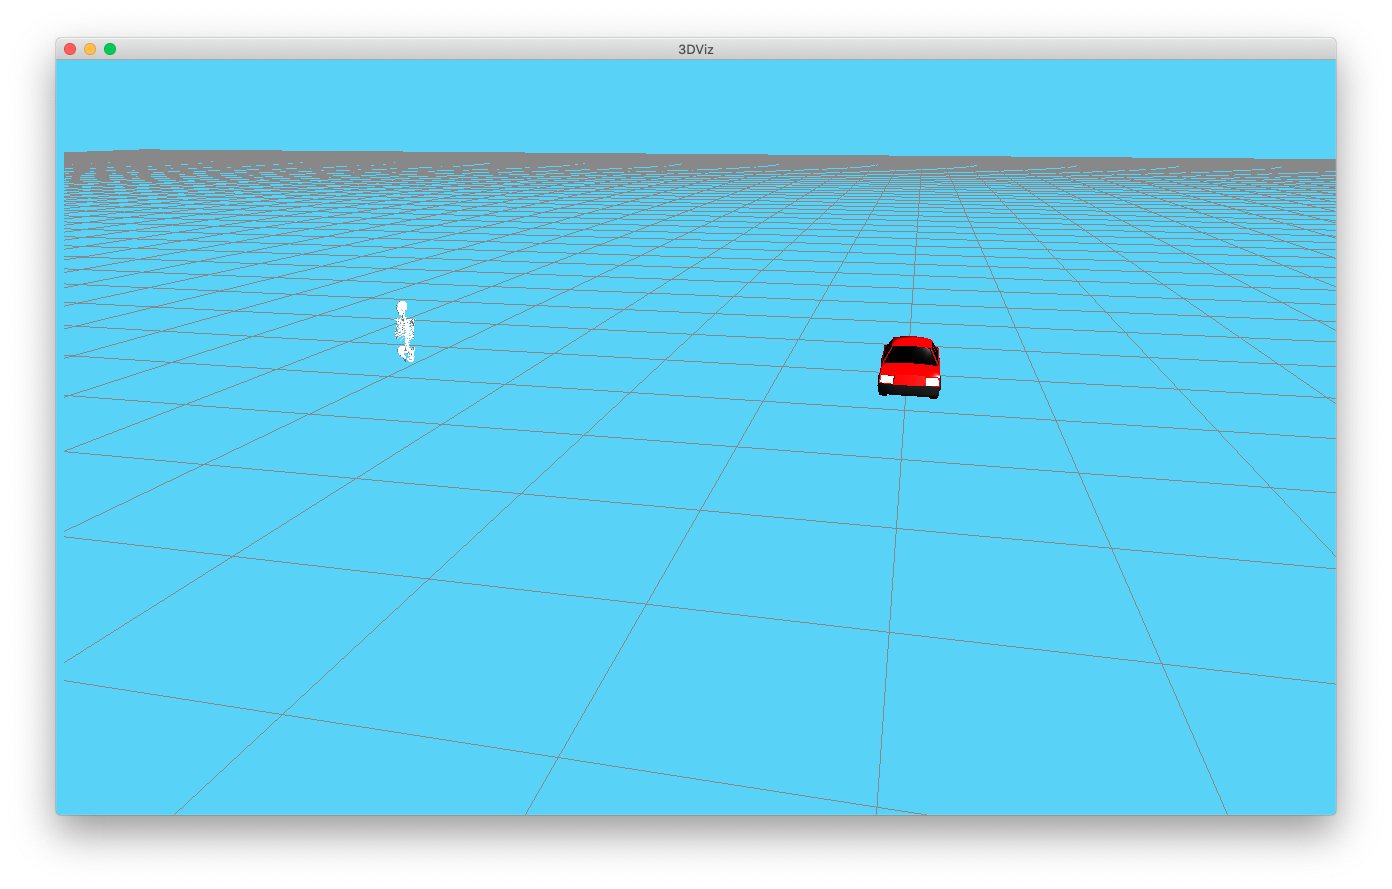
\includegraphics[width=0.8\textwidth]{figures/visualizarmodel.png}
		\caption{Objetos 3D mostrados en el visor}
		\label{fig.visualizarmodel}
		\end{center}
\end{figure}
\subsubsection{Mover los objetos 3D}
A diferencia de un punto o un segmento, que es más sencillo eliminarlo y volver a crearlo en la nueva posición, un objeto 3D nos interesa reubicarlo a la nueva posición en lugar de eliminarlo y crearlo de nuevo, lo que conllevaría tener que enviar una url o un texto plano con el archivo del objeto y cargarlo de nuevo, teniendo un retardo y carga de trabajo importante para el visor.

Al haber identificado el objeto mediante un id único (en el caso del punto y la recta, el id es el mismo para cada elemento), nos permite realizar el movimiento. Esto se realiza mediante la siguiente secuencia de código:
\begin{lstlisting}[frame=single]
function moveObj(objeto){
	selectedObject = scene.getObjectByName(objeto.id);
	selectedObject.position.set(objeto.x, objeto.z, objeto.y);
	selectedObject.rotation.set(objeto.rx*toDegrees, objeto.rz * toDegrees, 
							objeto.ry * toDegrees,);
}
\end{lstlisting}
Como se puede apreciar, mover el objeto es mucho más rápido y sencillo que eliminarlo y crearlo de nuevo. Primero seleccionamos el objeto mediante el identificador, posteriormente reubicamos el objeto seleccionado a las nuevas coordenadas y le aplicamos la nueva orientación. La imagen que se muestra a continuación corresponde a los objetos anteriores desplazados y rotados:
\begin{figure}[H]
  \begin{center}
    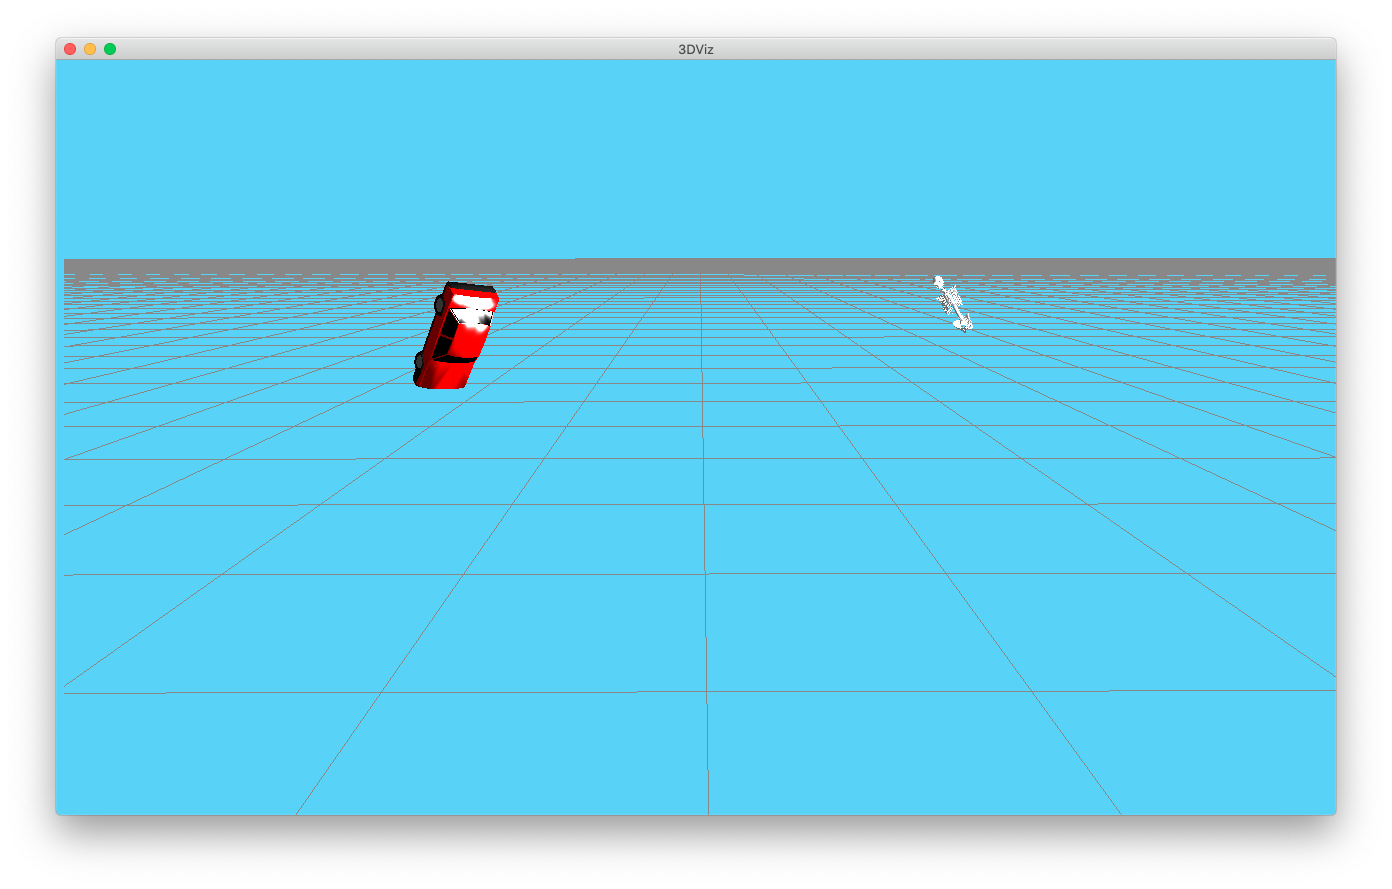
\includegraphics[width=0.8\textwidth]{figures/movermodelos.png}
		\caption{Objetos 3D reubicados y rotados}
		\label{fig.movermodelos}
		\end{center}
\end{figure}
\subsection{Borrar elementos mostrados en el visor}
Como ya se ha indicado anteriormente, el visor ofrece la posibilidad de eliminar todos los elementos que se están mostrando en ese momento en él, si así lo ha indicado el servidor cuando envía un nuevo elemento para mostrar. Eliminar todos los elementos de la escena es simple, el siguiente código elimina todos los elementos que hubiese en la escena:

\begin{lstlisting}[frame=single]
function deleteObj(){
	for (i = 0; i < id_list.length; i++){
		var selectedObject = scene.getObjectByName(id_list[i]);
		while (selectedObject != null) {
			scene.remove(selectedObject);
			selectedObject = scene.getObjectByName(id_list[i]);
		}
	}
}
\end{lstlisting}
En este código lo que se hace es recorrer el array con los identificadores de todos los objetos que hay en el visor y que se han ido añadiendo en el momento de incluir al visor los objetos (dado que los puntos y los segmentos tienen el mismo id, son añadidos a la lista de identificadores cuando se reciben los primeros elementos de cada tipo). Se selecciona el objeto en el visor que coincida con el identificador de la lista. Posteriormente se realiza otro bucle para eliminar todos los elementos del visor con ese identificador (esto se realiza para los segmentos y los puntos, que como ya se ha indicado, todos tiene el mismo).

\section{Mensajes}
En esta sección se describirá la estructura de los mensajes para cada tipo y como se definen utilizando el lenguaje de descripción Slice, explicado en el capitulo 3 de esta memoria. 
\subsection{Estructura del mensaje para visualizar los puntos}
Para representar un punto, como veremos en la siguiente sección, únicamente necesitamos una posición en el eje de coordenadas y el color que tendrá el punto. Teniendo en cuenta esto, la estructura del mensaje sería muy simple:
\begin{itemize}
\item Coordenada ``X''
\item Coordenada ``Y''
\item Coordenada ``Z''
\item Componente de color ``R'' (valor decimal entre 0 y 1)
\item Componente de color ``G'' (valor decimal entre 0 y 1)
\item Componente de color ``B'' (valor decimal entre 0 y 1)
\end{itemize}

Esta estructura es definida mediante el lenguaje Slice de la siguiente forma en el archivo ``primitives.ice'', que contendrá las definiciones de las estructuras intermedias creadas para definir estrucutras más complejas y definitivas :

\begin{lstlisting}[frame=single]
#ifndef PRIMITIVES_ICE
#define PRIMITIVES_ICE

module jderobot{
	struct RGBPoint{
      		float x;
      		float y;
      		float z;
      		float r;
      		float g;
      		float b;
	};
};
#endif
\end{lstlisting}

Sin embargo, como se ha explicado anteriormente, el visor tiene la iniciativa y solicitará si hay nuevos puntos que mostrar cada cierto periodo de tiempo. Dado que puede interesar que este periodo sea largo para evitar constantes peticiones y mayor carga de trabajo, se ha decidido que no solo se pueda enviar un punto en cada petición, sino que se pueda enviar un buffer de puntos. La estructura del mensaje por tanto no será una posición en el eje de coordenadas y el color, sino una colección variable de estos elementos (podrá ser uno o más).
Finalmente, para dar la posibilidad al servidor de indicar si desea añadir o eliminar lo que se muestra en ese momento en el visor (refrescar la escena que muestra el visor), al mensaje se le añade un booleano que valga True, si se desea eliminar lo que se muestra en ese momento y únicamente que se visualice lo que se transmite en ese mensaje, o False, si lo que se desea es añadir lo transmitido en este mensaje a lo que ya se muestra.
Por tanto el mensaje quedará como sigue:
\begin{itemize}
\item Buffer de puntos con los siguientes parámetros:
	\begin{itemize}
	\item Coordenada ``X''
	\item Coordenada ``Y''
	\item Coordenada ``Z''
	\item Componente de color ``R'' (valor decimal entre 0 y 1)
	\item Componente de color ``G'' (valor decimal entre 0 y 1)
	\item Componente de color ``B'' (valor decimal entre 0 y 1)
	\end{itemize}
\item Refresco del visor
\end{itemize}

Esta estructura final del mensaje con el buffer de puntos y el refresco estará definida en el archivo Slice ``visualization.ice'', donde se definen las estructuras definitivas de los mensajes, utilizando las primitivas creadas en el archivo ``primitives.ice'':

\begin{lstlisting}[frame=single]
#ifndef VISUALIZATION_ICE
#define VISUALIZATION_ICE

#include <primitives.ice>

module jderobot{

	sequence<RGBPoint> Points;

	struct bufferPoints{
		Points buffer;
		bool refresh;
	};
};
#endif
\end{lstlisting}


\subsection{Estructura del mensaje para visualizar segmentos}
Como se verá en la siguiente sección, para visualizar un segmento únicamente es necesario enviar la posición en el eje de coordenadas de dos puntos y el color con el que se desea visualizar el segmento. Por tanto, la estructura del mensaje para representar un segmento será la siguiente:
\begin{itemize}
\item Punto de inicio
	\begin{itemize}
		\item Coordenada ``X''
		\item Coordenada ``Y''
		\item Coordenada ``Z''
	\end{itemize}
\item Punto de fin
	\begin{itemize}
		\item Coordenada ``X''
		\item Coordenada ``Y''
		\item Coordenada ``Z''
	\end{itemize}
\item Componente de color ``R'' (valor decimal entre 0 y 1)
\item Componente de color ``G'' (valor decimal entre 0 y 1)
\item Componente de color ``B'' (valor decimal entre 0 y 1)
\end{itemize}

Se extiende el archivo ``primitives.ice'' para incluir las estructuras intermedias necesarias:

\begin{lstlisting}[frame=single]
structu Point{
	float x;
      	float y;
      	float z;
};

struct Segment{
	Point fromPoint;
	Point toPoint;
};


struct RGBSegment{
	Segment seg;
	float r;
	float g;
	float b;
};

\end{lstlisting}


Sin embargo, al igual que para el caso de los puntos, se desea poder enviar varios segmentos. El mensaje, por tanto, contendrá un buffer de segmentos cuya estructura será una colección de dos puntos, con su posición en el eje de coordenadas, y el color de cada segmento.
Finalmente, también se incluye el booleano para indicar si se debe refrescar el visor o por el contrario simplemente se deben añadir a lo que ya se muestra.
La estructura final del mensaje de envío de segmentos será la siguiente:
\begin{itemize}
	\item Buffer de segmentos
	\begin{itemize}
		\item Punto de inicio
		\begin{itemize}
			\item Coordenada ``X''
			\item Coordenada ``Y''
			\item Coordenada ``Z''
		\end{itemize}
		\item Punto de fin
		\begin{itemize}
			\item Coordenada ``X''
			\item Coordenada ``Y''
			\item Coordenada ``Z''
		\end{itemize}
		\item Componente de color ``R'' (valor decimal entre 0 y 1)
		\item Componente de color ``G'' (valor decimal entre 0 y 1)
		\item Componente de color ``B'' (valor decimal entre 0 y 1)
	\end{itemize}
	\item Refresco del visor
\end{itemize}

Ahora es necesario definir el formato definitivo del mensaje, para ello se extenderá el archivo ``visualization.ice'' de la siguiente forma:

\begin{lstlisting}[frame=single]
	
sequence<RGBSegment> Segments;
	
struct bufferSegments{
	Segments buffer;
	bool refresh;
};
\end{lstlisting}

\subsection{Estructura del mensaje para visualizar un objeto 3D}
En este caso, primero hay que indicar que el mensaje de petición es algo diferente a los casos anteriores. Mientras que para los segmentos y para los puntos únicamente se hace la petición sin añadir ningún parámetro a la misma (la forma de realizar la petición se detallará en secciones posteriores), en el caso de las peticiones de un objeto 3D desde el visor 3D al servidor, se le debe incluir el identificador que se le va a dar al objeto (en caso de que el servidor tenga uno para enviar), de modo que tanto visor como servidor puedan relacionar las peticiones de movimiento o borrado de un objeto mediante este identificador.
Una vez explicado esto, ya podemos ver cómo es la estructura del mensaje para visualizar un objeto 3D. Para mostrar un objeto, se necesita conoces el archivo que contiene el objeto, el formato del archivo, la posición en el eje de coordenadas, la orientación del objeto y la escala del objeto. 

El archivo puede ser enviado de dos formas, la primera forma es mediante una url a un servidor externo o página web, la segunda forma es enviar el fichero como texto plano, sin embargo esta segunda vía tiene el inconveniente de que no pueden ser enviados archivos de más de 1 MB de tamaño, por lo que si se quiere enviar un archivo más grande, debe realizarse mediante url.

El formato del archivo, como se explicará en próximas secciones, puede ser del tipo ``dae'' o ``obj''. Estos dos formatos son los más utilizados a la hora de crear objetos 3D y por tanto se considerá que dando soporte a los dos formatos permite usar cualquier objeto que se desee.

La escala del objeto será un número decimal que indicará el tamaño con el que se desea mostrar el objeto, permitiendo así mostrar varias veces el mismo objeto pero cambiando de tamaño (por ejemplo, podemos querer mostrar un brazo humano en diferentes tamaños para representar a un niño y a un adulto).

Por último, tanto para la posición como para la orientación se usará la clase ``Pose3D''. Esta clase esta formada por las coordenadas ``X'', ``Y'' y ``Z'', una componente ``h'' que no se utilizara, y los cuaterniones ``q0'', ``q1'', ``q2'' y ``q3'' para después usando las formulas matemáticas correspondientes y que se explicaran más adelante, nos proporciona la orientación del objeto.

Por tanto, el formato del mensaje tendrá la siguiente estructura:
\begin{itemize}
	\item Archivo con el objeto 3D
	\item Formato del archivo
	\item	Pose3D
	\begin{itemize}
		\item Coordenada ``X''
		\item Coordenada ``Y''
		\item Coordenada ``Z''
		\item ``h''
		\item Cuaternión ``q0''
		\item Cuaternión ``q1''
		\item Cuaternión ``q2''
		\item Cuaternión ``q3''
	\end{itemize}
	\item Escala
	\item Identificador
	\item Refresco del visor
\end{itemize}
Como se puede ver, se vuelve a enviar el identificador que había sido previamente transmitido por el visor, y se añade también el refresco al igual que para los puntos y los segmentos. Sin embargo, debido a las limitaciones de tamaño de los archivos que se pueden enviar mediante ICE, y la necesidad de establecer un identificador común, solo es posible enviar un objeto 3D por petición realizada y no un buffer de objetos, como si podemos hacer con los puntos y los segmentos.

La clase ``Pose3D'' es definida en un nuevo archivo Slice llamado ``pose3d.ice'':

\begin{lstlisting}[frame=single]
#ifndef POSE3D_ICE
#define POSE3D_ICE

module jderobot{

  class Pose3DData
  {
		float x;
		float y;
		float z;
  		float h;
		float q0;
		float q1;
		float q2;
		float q3;
  };

}; 
#endif
\end{lstlisting}

Este mensaje quedará definido en el archivo Slice ``visualization.ice'', al tratarse de un formato final y no de una primitiva (se trata de una estructura de mensaje final y no una estructura intermedia para crear nuevas). Además, es necesario incluir al principio la referencia al archivo `pose3d.ice'':

\begin{lstlisting}[frame=single]

#include <pose3d.ice>
	....
  	struct object3d {
    		string obj;
    		string id;
    		string format;
    		float scale;
    		Pose3DData pos;
    		bool refresh;
  	};

 \end{lstlisting}


\subsection{Estructura del mensaje para mover los objetos 3D}
Como se explicará en secciones sucesivas, los objetos 3D que se visualizan probablemente se deseen moverlos de posición u orientación y borrarlos y crearlos de nuevo implica un mayor retardo y carga de trabajo, por lo que ha sido necesario incorporar una secuencia de petición y envío de movimiento, pero solo se comenzará a realizar la petición de movimiento una vez se muestre un objeto ya en el visor. La estructura de este mensaje será una versión reducida del mensaje para crear un objeto. En este caso únicamente se deberá enviar la nueva posición mediante la clase ``Pose3D'' y el identificador del objeto que se desea mover. Por tanto, la estructura quedará de la siguiente manera:
\begin{itemize}
	\item	Pose3D
	\begin{itemize}
		\item Coordenada ``X''
		\item Coordenada ``Y''
		\item Coordenada ``Z''
		\item ``h''
		\item Cuaternión ``q0''
		\item Cuaternión ``q1''
		\item Cuaternión ``q2''
		\item Cuaternión ``q3''
	\end{itemize}
	\item Identificador
\end{itemize}

Este mensaje queda definido en el archivo ``visualization.ice'', al tratarse de un movimiento y no de un elemento nuevo:

\begin{lstlisting}[frame=single]

struct PoseObj3D{
    	Pose3DData pos;
	string id;
 };
\end{lstlisting}

En este caso, se vuelve a poder enviar una secuencia de movimientos para uno o más objetos, por lo que, al no tener el impedimento del tamaño de los archivos o del identificador, se decide permitir el envío de buffers con estas secuencias de movimiento de manera que si entre petición y petición, se ha movido un objeto varias veces o se han movido varios objetos que se muestran en el visor, se pueda realizar esos movimientos al mismo tiempo en el visor, evitando largos retardos que provocarían enviar los movimientos de uno en uno. Sin embargo, como es evidente, en esta ocasión el refresco no se envíe al no tener sentido eliminar todo lo que se muestra en la escena, sí estamos enviando la actualización de algo que se muestra en la escena. Teniendo en cuenta esto, la estructura final del mensaje será la siguiente:
\begin{itemize}
	\item Buffer de movimientos
	\begin{itemize}
		\item	Pose3D
		\begin{itemize}
			\item Coordenada ``X''
			\item Coordenada ``Y''
			\item Coordenada ``Z''
			\item ``h''
			\item Cuaternión ``q0''
			\item Cuaternión ``q1''
			\item Cuaternión ``q2''
			\item Cuaternión ``q3''
		\end{itemize}
		\item Identificador
	\end{itemize}
\end{itemize}

El mensaje final queda definido de la siguiente forma en el archivo ``visualization.ice'':

\begin{lstlisting}[frame=single]

sequence<PoseObj3D> bufferPoseObj3D;

\end{lstlisting}

\section{Conexiones}
En esta sección se va a tratar cómo se realiza la conexión y la posterior recepción de cada uno de los objetos y objetos 3D anteriormente indicados. La conexión se realizará mediante el middleware ICE, explicado en capítulos anteriores, y su lenguaje de especificación Slice nombrando a los ficheros creados con este lenguaje interfaces slice. Lo primero que se detallará en este capitulo serán estas interfaces, ya que son la base de la conexión y que tanto el servidor como el visor deben compartir. Si alguna de las dos partes no usan la misma interfaz, la conexión no podrá llevarse a cabo correctamente. Después, se detallará como se realiza la conexión con el servidor y la posterior petición de cada tipo de objeto. Finalmente, se explicará cómo se realiza la recepción de cada objeto y el tratamiento que recibe cada uno para su posterior visualización en el visor mediante las funciones indicadas en la anterior sección.

\subsection{Conexión y peticiones al servidor}
Lo primero que hay que indicar es que para la conexión e intercambios con el servidor, el visor hace uso de los Web Workers de HTML5 \footnote{\url{https://www.w3schools.com/html/html5_webworkers.asp}} que permite realizar ejecuciones en segundo plano sin bloquear al proceso principal. Su uso es imprescindible para que el hilo principal no se bloquee y pueda mostrar los elementos que se reciban mientras espera la recepción del resto de peticiones realizadas.

Una vez que el visor se ha lanzado y se ha terminado de cargar, se crear el Web Worker y se envía el mensaje para que se establezca la conexión, esto se realiza utilizando el siguiente código:
\begin{lstlisting}[frame=single]
w = new Worker("js/3DViz_worker.js");
w.postMessage({func:"Start",server:config.Server, port:config.Port});
\end{lstlisting}

Cuando se ha creado el Worker, se inicializa la conexión ICE que devuelve un objeto ``Ice.Communicator'', que es el objeto principal para establecer una comunicación ICE. Posteriormente se crea un objeto con la interfaz indicada anteriormente para poder realizar la conexión. También se incializan las variables para posteriormente lanzar el Promise (permite manejar la naturaleza asíncrona de ICE) y la variable donde se guardará el proxy con la conexión realizada con el servidor. Esto se realiza mediante las siguientes sentencias:
\begin{lstlisting}[frame=single]
var ic = Ice.initialize();
var communicator;
var Promise;
var Prx = jderobot.VisualizationPrx;
var srv;
\end{lstlisting}

Una vez incializada la conexión ICE, creado el objeto con la interfaz y recibido en el Worker el mensaje para que se establezca la conexión, se comienza el proceso para realizarla. Lo primero que se debe realizar es crear el endpoint mediante la ip y el puerto indicado en el fichero de configuración, después se crea un proxy realizando una petición al servidor mediante la llamada a ``stringToProxy'', pasándole como parámetro una cadena de texto que contiene la identidad del objeto (será a partir de la cual el servidor sea capaz de identificar a que proxy se está intentando conectar el cliente) y el endpoint. El proxy que nos devuelve es del tipo ``Ice.ObjectPrx'', pero realmente lo que se necesita es un proxy a la interfaz creada en ``visualization.ice'', que se hará mediante una petición Promise, el objeto con la interfaz y el proxy que se acaba de recibir. Esta petición lo que hace es preguntar al servidor si el proxy que nos ha devuelto es un proxy para el objeto de la interfaz de ``visualization.ice'', si lo es nos devuelve un proxy del tipo ``jderobot.VisualizationPrx'' que guardamos en la variable creada para almacenar la conexión, sino, devolverá un error.  Finalmente, el Worker manda un mensaje al hilo principal indicando que la conexión se ha realizado correctamente. El siguiente código muestra como se realiza todo lo indicado anteriormente:

\begin{lstlisting}[frame=single]
function connect(server,port){
  endpoint = "ws -h " + server + " -p " + port;
  var proxy = ic.stringToProxy("3DViz:" + endpoint);
  Promise = Prx.checkedCast(proxy).then(
      function(printer)
      {
          srv = printer;
          self.postMessage({func:"Connect"});
      });
}
\end{lstlisting}

Cuando el hilo principal recibe el mensaje indicando que la conexión ha sido exitosa, establece las llamadas periódicas (utilizando el tiempo indicado en el fichero de configuración) a las funciones que se encargan de realizar las peticiones al servidor mediante el método de HTML ``setInterval()'' \footnote{\url{https://www.w3schools.com/jsref/met_win_setinterval.asp}} , si no lo ha sido elimina el Worker e imprime el mensaje por consola. Esto se realiza de la siguiente manera:

\begin{lstlisting}[frame=single]
w.onmessage = function(event) {
      	 if (event.data.func == "Connect"){
		pointInterval = setInterval(function(){
					setPoint();
						}, config.updatePoints);
		lineInterval = setInterval(function(){
					setLine();
					},config.updateSegments);
		objInterval = setInterval(function(){
					setObj();
					},config.updateModels);}	
        } else {
          console.log(event.data);
          w.terminate();
        }
\end{lstlisting}

Cuando se pase el tiempo, se activa las funciones que envían el mensaje al Worker para que realice las peticiones al servidor. Estas peticiones serán para todos los objetos igual salvo en el caso de la petición de los objetos 3D, que como se ha explicado anteriormente, enviará el identificador que se dará al objeto en caso de que haya uno. Este identificador será una cadena de ``obj'' y un contador de objetos que hay en la escena, es decir, si no hay objetos en la escena, el siguiente tendrá de identificador ``obj1'', el siguiente ``obj2'' y así sucesivamente. Finalmente, esta función terminará realizando una llamada a la función que se encargará de gestionar las respuestas del servidor. A continuación se muestran estas funciones:

\begin{lstlisting}[frame=single]
function setPoint(){
      w.postMessage({func:"setPoint"});
      getData();
}
function setLine(){
	w.postMessage({func:"setLine"});
	getData();
}
function setObj(){
	id = "obj" + cont;
	w.postMessage({func:"setObj", id: id});
	getData();
}
\end{lstlisting}

En el Worker, cuando se reciba los mensajes para que se soliciten cada tipo de elemento al servidor, se realiza la petición usando el proxy con la conexión y las funciones definidas en la interfaz Slice explicada anteriormente. Si a la petición se recibe respuesta, se reenvía al hilo principal para su manejo. A continuación se muestran estas peticiones:

\begin{lstlisting}[frame=single]
function setPoint(point){
 	srv.getPoints().then(function(data){
		self.postMessage({func:"drawPoint",points: data});
	});
}

function setLine(){
	srv.getSegment().then(function(data){
      		self.postMessage({func:"drawLine", segments: data});
  	});
}

function setObj(id){
  	srv.getObj3D(id).then(function(data){
    		self.postMessage({func:"drawObj", obj: data});
  	});
}
\end{lstlisting}

Como se puede ver, solo se esta realizando las peticiones para los puntos, los segmentos y los objetos, pero no para los movimientos de los objetos, ya que solo se realiza una vez que se ha recibido un objeto para mostrar. Una vez que se tiene un objeto, se activa la llamada periódica a la función para que envíe el mensaje al Worker para que se realice la petición al servidor de la misma forma que las demás.

Las funciones para realizar las peticiones al servidor, se han tenido que definir previamente mediante el lenguaje de descriptivo de ICE, Slice. Por tanto, para realizar la definición, se ha extendido el archivo ``visualization.ice'' explicado en la sección sobre los mensajes. A este archivo se le añade los siguiente:

\begin{lstlisting}[frame=single]

interface Visualization
	{
	      bufferSegments getSegment ();
	      bufferPoints getPoints();
	      object3d getObj3D(string id);
	      bufferPoseObj3D getPoseObj3DData();
	};
};

\end{lstlisting}

\subsection{Recepción y tratamiento de los mensajes recibidos}
Ya se ha explicado cómo se conecta, se envían los mensajes de petición al servidor y se recepciona la respuesta en el Worker que la transmite al hilo principal. Ahora se explicará cómo se trata esos mensajes el hilo principal para mostrarlo en el visor.

En el hilo principal hay un manejador de mensajes que será la función ``getData()'' que se invoca cada vez que se realiza una petición, como se indicó anteriormente. En esta función se analiza el mensaje que se recibe procedente del Worker. Se revisa cuál es el tipo y se realizan las tareas previas necesarias para posteriormente visualizar el elemento usando los métodos explicados en la sección sobre la interfaz gráfica. El siguiente condicional es el encargado de realizar este análisis:

\begin{lstlisting}[frame=single]
function getData (){
	w.onmessage = function(event) {
		if (event.data.func == "drawPoint"){
			...
		} else if (event.data.func == "drawLine"){
			...
		} else if (event.data.func == "drawObj") {
			...
		} else if (event.data.func == "pose3d") {
			...
		}
	}
}
\end{lstlisting}

\subsubsection{Tratar los puntos}
Si el mensaje enviado por el Worker es del tipo ``drawPoint'', el manejador indicará que se deben ejecutar las sentencias correspondientes a la visualización de los puntos. Una vez concluido que se deben mostrar los puntos, lo primero que se realiza es verificar si el servidor ha solicitado que haya refresco del visor o no, si el servidor ha indicado 	que se debe refrescar el visor (y si el mensaje trae puntos que mostrar, ya que, sino, se interpretará el mensaje como erróneo), se llama al método encargado de eliminar los elementos que se muestran en ese momento en el visor y que se describió en la sección sobre la interfaz gráfica. Tanto si se ha refrescado como si no, se recorre el buffer de puntos mediante un bucle ``for'', invocando al método encargado de mostrar un punto en el visor, en cada iteración hasta que ya no queden más puntos para mostrar. Al método se le pasa por parámetros el punto completo (coordenadas y componentes RGB), ya que como vimos anteriormente, el método ya se encarga de diferenciar cada uno y realizar las tareas necesarias para mostrarlos. El siguiente código es el encargado de realizar estas funciones:

\begin{lstlisting}[frame=single]
else if (event.data.func == "drawPoint"){
	if (event.data.points.refresh & (event.data.points.buffer.length != 0)){
		deleteObj();
	}
	points = event.data.points.buffer;
	for (var i = 0; i < points.length; i+=1) {
        		addPoint(points[i]);
	}
}
\end{lstlisting}

\subsubsection{Tratar los segmentos}
El tratamiento de los mensajes que contienen los segmentos es muy similar a los mensajes con los puntos. Se revisa si es necesario refrescar el visor o no, si así lo fuera se elimina los elementos que hay en el visor (si los hubiese), posteriormente se recorre el buffer de segmentos mediante el bucle ``for'' y finalmente se llama al método para mostrar segmentos en cada iteración. Al igual que en el caso de los puntos, se pasa como parámetro el segmentos completos y ya se encarga el método de separarlo y realizar las tareas correspondientes. El siguiente código muestra como realizar esto, pudiéndose apreciar que es muy similar al caso de los puntos:

\begin{lstlisting}[frame=single]
if (event.data.func == "drawLine"){
	if (event.data.segments.refresh & (event.data.segments.buffer.length !=0)){
		deleteObj();
	}
	segments = event.data.segments.buffer;
	for (var i = 0; i < segments.length; i+=1) {
		addLine(segments[i], "segments");
	}
}
\end{lstlisting}

\subsubsection{Tratar los objetos 3D}
El tratamiento de los objetos 3D comienza de la misma forma que los otros dos elementos, es decir, se debe revisar si requiere refresco, o no, del visor. Sin embargo, una vez que se ha borrado, o no, el contenido del visor, se actualiza el contador que forma el identificador que se ha indicado en las secciones anteriores. Posteriormente, es necesario realizar la conversión de la ubicación y orientación enviada como ``Pose3D'' a un formato que el método encargado de mostrar los objetos sea capaz de entender.

Para realizar esta conversión, lo primero que se realiza es crear una clase de JavaScript cuya estructura contendrá los parámetros que se necesitan para mostrar el objeto, es decir la posición en el eje de coordenadas (coordenadas ``x'', ``y'' y ``z''), las orientaciones en cada eje de coordenadas (orientación ``rx'', ``ry'' y ``rz'') y el identificador del objeto 3D. La clase queda por tanto del siguiente modo:
\begin{lstlisting}[frame=single]
class obj3DPose {
	constructor(id, x, y, z, rx, ry, rz){
		this.id = id;
		this.x = x;
		this.y = y;
		this.z = z;
		this.rx = rx;
		this.ry = ry;
		this.rz = rz;
	}
}
\end{lstlisting}

Para realizar la conversión, se han credo tres métodos diferentes que devolverán cada uno de ellos la orientación en cada uno de los ejes de coordenadas. Estos métodos usarán las formulas matemáticas que transforman los cuatriones en los ángulos de navegación usados para describir la orientación de un objeto tridimensional y que son un tipo de ángulos de Euler \footnote{\url{https://en.wikipedia.org/wiki/Conversion_between_quaternions_and_Euler_angles}}. Este sistema es muy utilizado en navegación de los aviones y drones, y están formados por la dirección (``yaw''), elevación (``pitch'') y ángulo de alabeo (``roll'') correspondiendo respectivamente a la orientación en el eje ``z'', el eje ``y'' y el eje ``z''. Estas formulas matemáticas incorporadas a nuestro código origina los siguientes métodos:

\begin{lstlisting}[frame=single]

function getYaw(q0,q1,q2,q3) {
       var rotateZa0=2.0*(q1*q2 + q0*q3);
       var rotateZa1=q0*q0 + q1*q1 - q2*q2 - q3*q3;
       var rotateZ=0.0;
       if(rotateZa0 != 0.0 && rotateZa1 != 0.0){
           rotateZ=Math.atan2(rotateZa0,rotateZa1);
       }
       return rotateZ;
}

function getRoll(q0,q1,q2,q3){
       rotateXa0=2.0*(q2*q3 + q0*q1);
       rotateXa1=q0*q0 - q1*q1 - q2*q2 + q3*q3;
       rotateX=0.0;

       if(rotateXa0 != 0.0 && rotateXa1 !=0.0){
           rotateX=Math.atan2(rotateXa0, rotateXa1);
       }
       return rotateX;
}
function getPitch(q0,q1,q2,q3){
       rotateYa0=-2.0*(q1*q3 - q0*q2);
       rotateY=0.0;
       if(rotateYa0>=1.0){
           rotateY=Math.PI/2.0;
       } else if(rotateYa0<=-1.0){
           rotateY=-Math.PI/2.0
       } else {
           rotateY=Math.asin(rotateYa0)
       }

       return rotateY;
}
\end{lstlisting}

Finalmente, se crea una función que devuelve un objeto de la nueva clase creada y que tienen ya la conversión. A esta función se le pasa por parámetro el objeto completo recibido y, mediante la llamada a las funciones para realizar la conversión, crea el objeto de la nueva clase que contendrá el identificador, las coordenadas ``x'', ``y'' y ``z'', sin ningún tipo de conversión, y las orientaciones en cada eje convertidas y que están en radianes. Esta función es la siguiente:

\begin{lstlisting}[frame=single]
function getPose3D(data){
	var rotateZ=getYaw(data.pos.q0, data.pos.q1, data.pos.q2, data.pos.q3);
	var rotateY=getPitch(data.pos.q0, data.pos.q1, data.pos.q2, data.pos.q3);
	var rotateX=getRoll(data.pos.q0, data.pos.q1, data.pos.q2, data.pos.q3);
	var objpose3d = new obj3DPose(data.id, data.pos.x, data.pos.y,
						data.pos.z, rotateX, rotateY, rotateZ);
	return objpose3d;
}
\end{lstlisting}

Una vez que ya hemos realizado la conversión, se llama al método encargado de cargar los objetos en el visor y que se explicó en la sección correspondiente. A este método, se le pasa por parámetro el objeto completo recibido del servidor y el objeto de la nueva clase que incorpora la conversión de la orientación, para que pueda mostrar el objeto en el visor. Tras ello, se arranca la petición periódica de movimientos para el objeto (si no estaba arrancada previamente) al tener ya mínimo un objeto para mover. Las siguientes sentencias hacen que tenga lugar todo lo indicado:

\begin{lstlisting}[frame=single]
else if (event.data.func == "drawObj") {
	if (event.data.refresh & (event.data.obj != "")){
		deleteObj();
	}
	cont += 1
	var pos = getPose3D(event.data.obj);
	addObj(event.data.obj,pos);
	if (posInterval == null){ 
		posInterval = setInterval(function(){
					setPose3D();
				}, config.updatePose3D);
	}
}
\end{lstlisting}

\subsubsection{Tratar el movimiento de los objetos}
En el caso de los mensajes con el movimiento, al no indicar si hay que refrescar el visor o no, únicamente se recorrerá buffer que contiene todos los movimientos realizando la conversión de Pose3D al formato admitido explicado anteriormente e invocando al método que realiza el movimiento de los objetos explicado en la sección sobre la interfaz gráfica. Cabe indicar que en la clase que se ha creado para la conversión se incluye el identificador del objeto que se va a mover, ya que, a diferencia de cuando invocamos al método que representa el objeto en el visor que se pasaba por parámetro el mensaje completo recibido del servidor y la nueva clase, en este caso solo pasamos por parámetro la nueva clase por lo que es necesario incluir el identificador. El código que se muestra este código:

\begin{lstlisting}[frame=single]
else if (event.data.func == "pose3d") {
	for (var i = 0; i < event.data.bpose3d.length; i += 1){
		data = event.data.bpose3d[i];
		var objpose3d = getPose3D(data);
		moveObj(objpose3d);}
	}
}
\end{lstlisting}

\section{Experimentos}
El visor está preparado para ser usado principalmente con Electron, ya que la lectura del fichero de configuración solo esta habilitada para sí se usa con Electro. Se puede utilizar en el navegador, pero la configuración será la que se indica al visor por defecto, no pudiendo modificarse lo que limita en gran manera las funciones del mismo.

Ejecutarlo con Electron se realiza de la misma manera que se explicó en el capitulo 3, por lo que se considerá que no es necesario repetir el proceso de adaptación de la aplicación para ser usada con Electron.

Para ejecutar el visor 3D y realizar pruebas, se ha creado un servidor de test escrito en python que enviará todos los tipos de elementos y movimientos, enviando valores aleatorias. En cada mensaje podrá envía entre 1 y 5 puntos y rectas, está preparado para enviar 3 objetos (uno en forma de texto plano y dos desde una url) y movimientos aleatorios para esos objetos.

\begin{enumerate}
\item En un terminal ejecutar el servidor de prueba:
\begin{lstlisting}[frame=single]
python server_test.py
\end{lstlisting}
\item En otro terminal, instalar Electron y las dependencias del visor:
\begin{lstlisting}[frame=single]
npm install
\end{lstlisting}
\item En el mismo terminal, ejecutar el visor 3D con Electron:
\begin{lstlisting}[frame=single]
npm start
\end{lstlisting}
\end{enumerate}

A continuación se muestra la prueba realizada con el servidor:

\begin{figure}[H]
  \begin{center}
    \subfigure[Visor 3D]{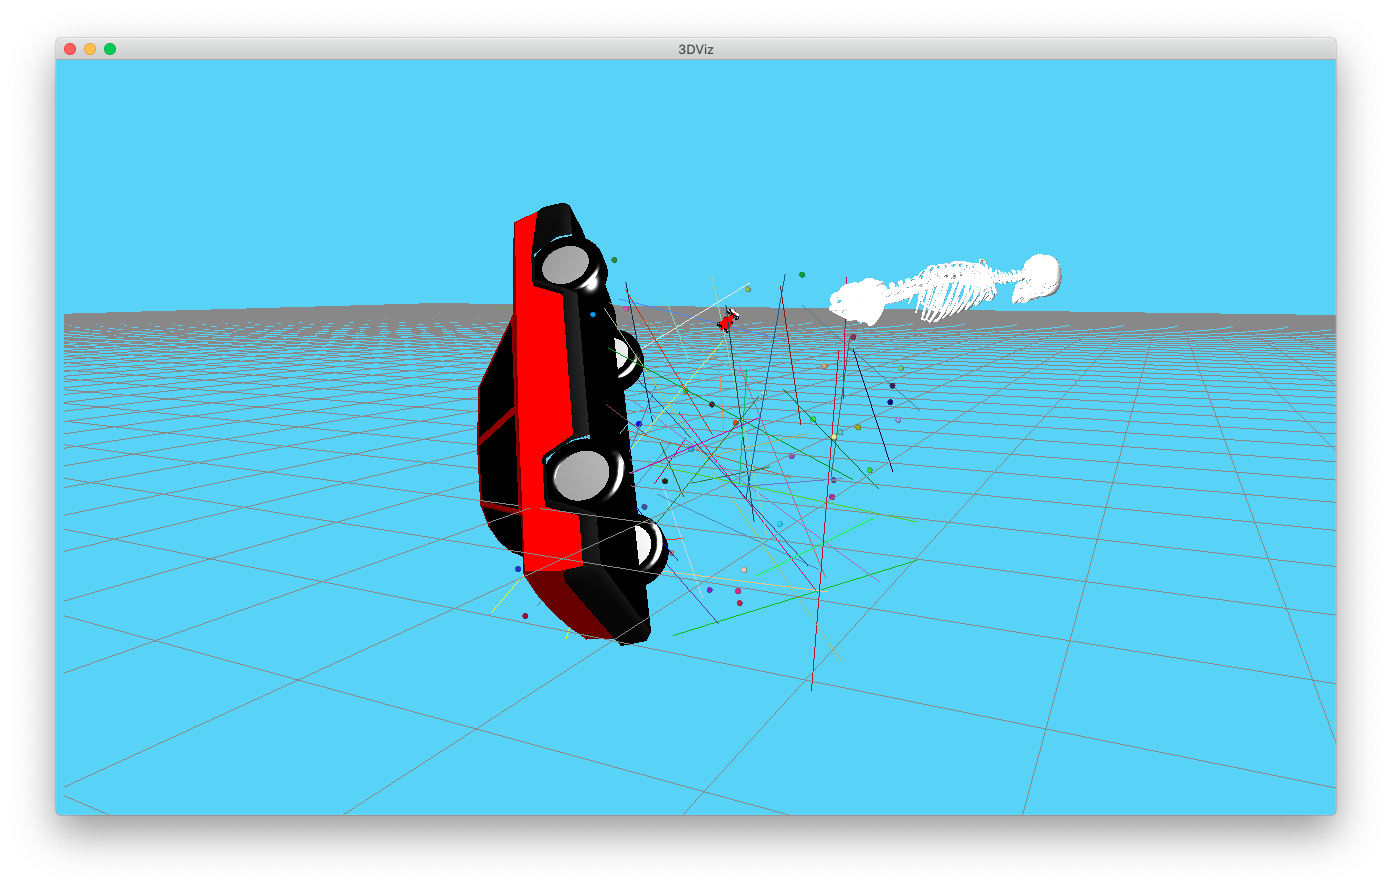
\includegraphics[width=0.4\textwidth]{figures/prueba3dviz.png}}
    \subfigure[Servidor de prueba]{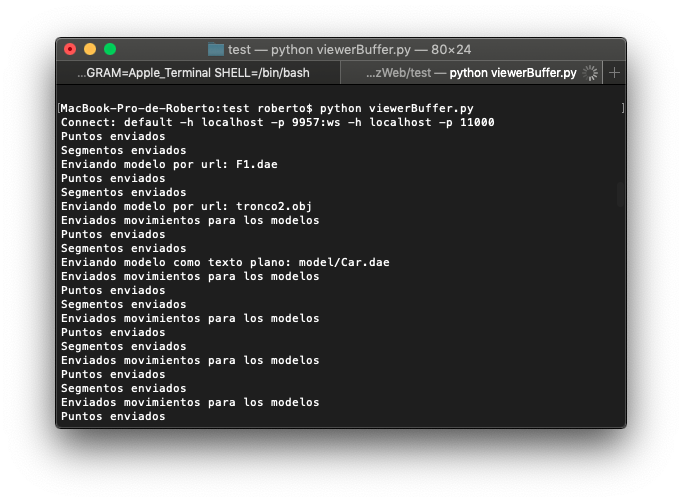
\includegraphics[width=0.4\textwidth]{figures/servertest3dviz.png}}
    \caption{Ejemplo de ejecución del visor con el servidor de prueba}
     \label{fig.ejemplo3dviz}
     \end{center}
\end{figure}












